\renewcommand*{\arraystretch}{1.1}

\subsection*{BI / read / 21}
\label{sec:bi-read-21}

\noindent\begin{tabularx}{\queryCardWidth}{|>{\queryPropertyCell}c|X|}
	\hline
	query & BI / read / 21 \\ \hline
%
	title & Zombies in a country \\ \hline
%
    pattern & \hfill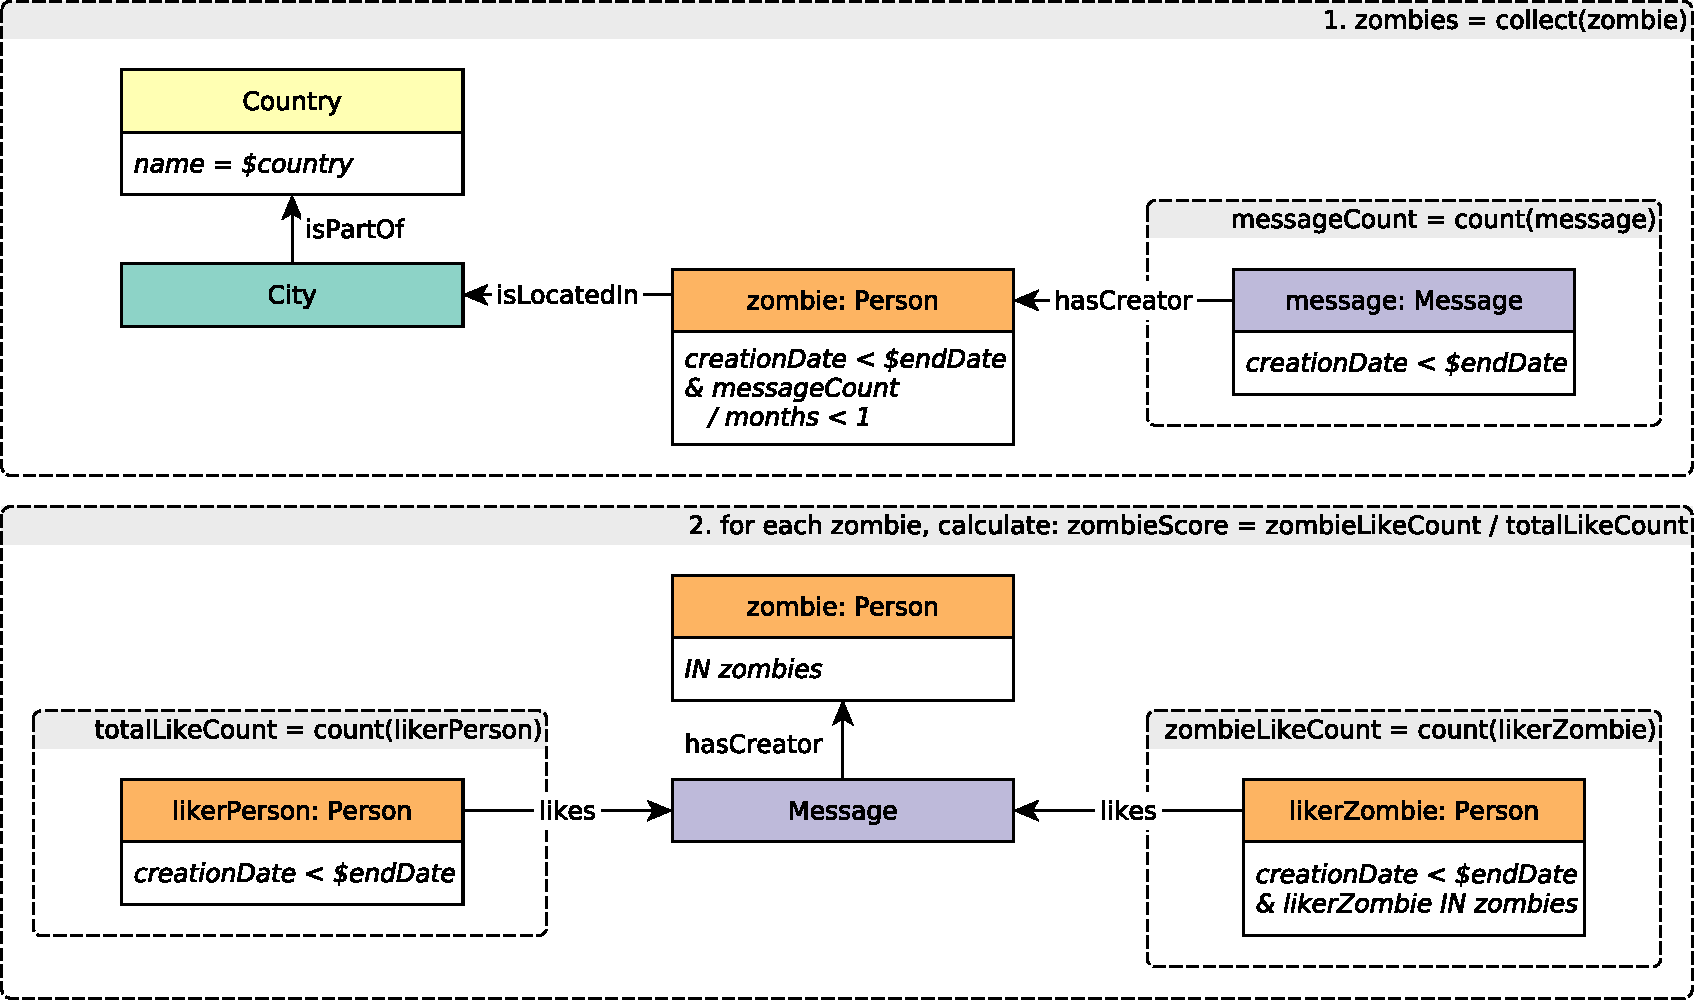
\includegraphics[scale=\patternscale,margin=0cm .2cm]{patterns/bi-read-21}\hfill\vadjust{} \\ \hline
%
	desc. & Find zombies within the given country, and return their zombie scores.

A zombie is a Person created before the given \texttt{endDate} and that
has created between \texttt{{[}0,\ 1)} Messages per month, on average,
during the time range between profile creation date and the given
\texttt{endDate}.

The number of months spans the time range from creation date of the
profile to the \texttt{endDate} and also includes partial months.
 \\ \hline
%
	
%
    
        params &
        \innerCardVSpace{\begin{tabularx}{\attributeCardWidth}{|>{\paramNumberCell}c|>{\varNameCell}M|>{\typeCell}m{\typeWidth}|Y|} \hline
        \cellcolor{parameter} \color{white} \footnotesize $\mathsf{1}$ &country& String &  \\ \hline
        \cellcolor{parameter} \color{white} \footnotesize $\mathsf{2}$ &endDate& Date &  \\ \hline
        \end{tabularx}}\innerCardVSpace \\ \hline
	
%
	
        result &
        \innerCardVSpace{\begin{tabularx}{\attributeCardWidth}{|>{\resultNumberCell}c|>{\varNameCell}M|>{\typeCell}m{\typeWidth}|>{\resultOriginCell}c|Y|} \hline
        $\mathsf{1}$ & person.id & 64-bit Integer &R&
                 \\ \hline
        $\mathsf{2}$ & zombieLikeCount & 32-bit Integer &A&
                 \\ \hline
        $\mathsf{3}$ & realLikeCount & 32-bit Integer &A&
                I think this should be `totalLikeCount` -- szarnyasg \\ \hline
        $\mathsf{4}$ & zombieScore & 32-bit Float &A&
                the ratio between the number of likes received from zombies (`zombieLikeCount`) and the total number of likes received on that person's messages (`realLikeCount`) -- only count likes received from profiles that were created before the given `endDate`. \\ \hline
        \end{tabularx}}\innerCardVSpace \\ \hline
	
%
	sort        &
        \innerCardVSpace{\begin{tabular}{|>{\sortNumberCell}c|>{\varNameCell}l|>{\directionCell}c|} \hline
        $\mathsf{1}$ & zombieScore & $\desc$ \\ \hline
        $\mathsf{2}$ & person.id & $\asc$ \\ \hline
        \end{tabular}}\innerCardVSpace \\ \hline
	%
	limit & 100 \\ \hline
	%
	CPs &
	\multicolumn{1}{>{\raggedright}l|}{
	    \chokePoint{1.2}, 
	    \chokePoint{2.1}, 
	    \chokePoint{2.3}, 
	    \chokePoint{2.4}, 
	    \chokePoint{3.2}, 
	    \chokePoint{3.3}, 
	    \chokePoint{5.1}, 
	    \chokePoint{5.3}
	    } \\ \hline
	%
    %
\end{tabularx}
\queryCardVSpace